\subsection{Software Design}
This section covers the bulk of our software design in the report as we mainly create artifacts in this sprint to help us during coding. First, we’ll show how we use UML artifacts to gain insight into complicated methods and tasks our system should support. Then we’ll describe and discuss how we use the GRASP principles \cite[p.~271, p.~413]{OOAD}. And finally, we’ll highlight the use of some design patterns not included in GRASP but relevant to our non-functional requirements.
\subsubsection{Static Object Modelling}
As described earlier, we try to model our system in a Client-Server pattern. While a user can store all his files offline, the remote storage should avoid redundancy and thus only store each file once no matter how many users are sharing it. This means that a client’s representation of a file should differ from the server. Additionally, even though the system is meant to be a proof of concept, we want to design modules for extensibility. This means that including support for other files than documents (say, binary files of any sort) should be easy to implement in a future release. We design with this in mind when doing our database design and thus our corresponding ‘mapped objects’. Below is a ‘class diagram’ modeling our database entities:\\
\begin{figure}[h]
  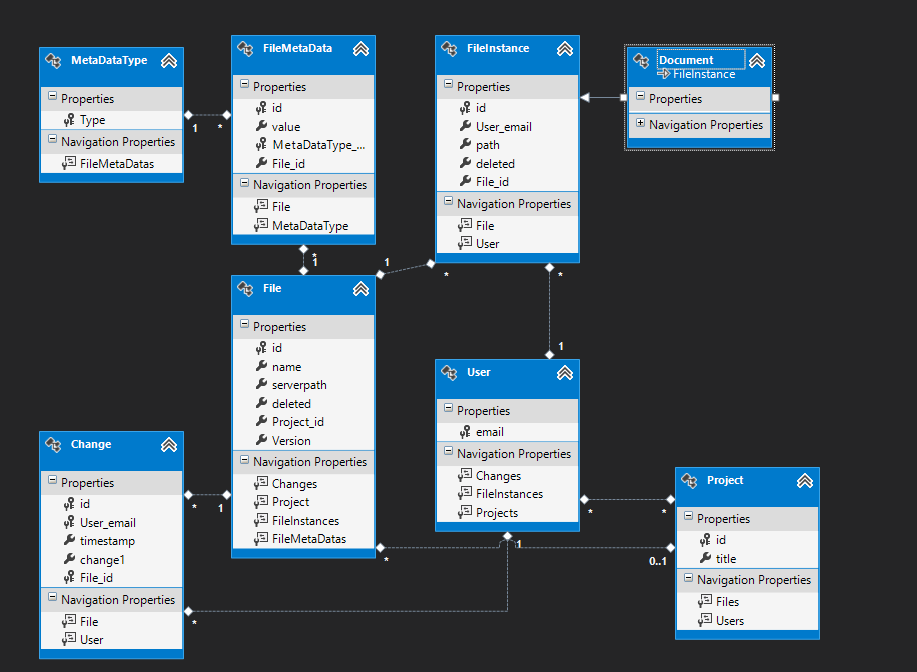
\includegraphics[width=\textwidth,natwidth=793,natheight=635]{illustrations/entitymodel.png}
  \caption{Entity Model}
  \label{entitymodel2}
\end{figure}
Although the model is more resembling to a relational model than an actual UML class diagram, we still find it useful in regards to describing our way of persisting data. Each File has a list of changes, which record a user, a time and a description of the change. Each File list to a number of FileInstances, which contains user-specific file information. A Document entity, which we use in the program to edit and show text, inherits directly from FileInstance. Additionally, each File contains a number of FileMetaData, which can be specific for the type of file.\\
The model does not describe any properties of the classes, as they almost only contain data. Only methods that represents the data as a text string is contained.
\subsubsection{Static Persistence View}
When designing the persistence part of the model, we initially build a list of interfaces so other parts of the system such as a controller or a network module can develop and compile their code against the persistence module. These interfaces are modeled in Visual Studio so we also can generate method signatures and classes from the definitions. A part of the interface diagram is shown below:\\
\begin{figure}[h]
  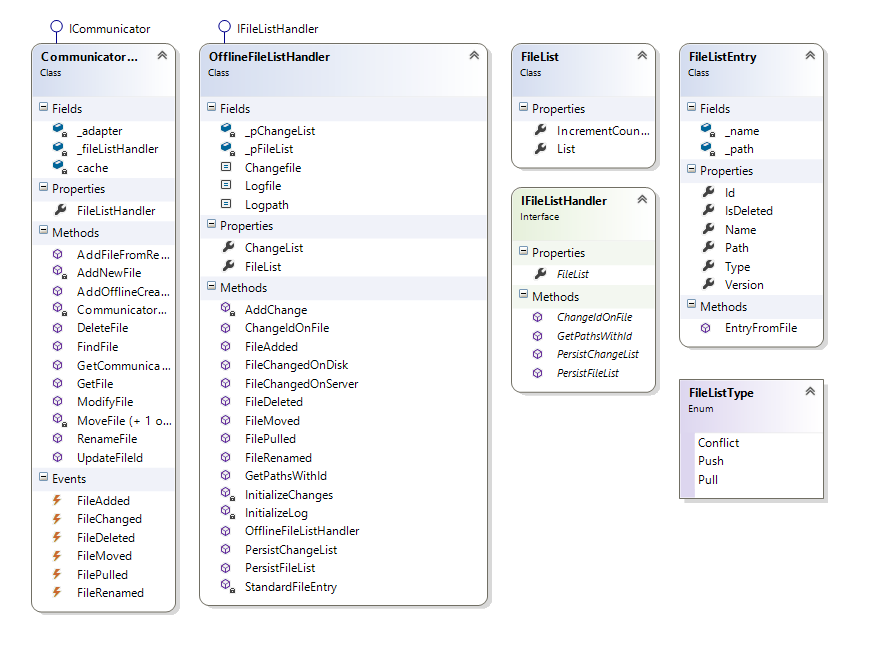
\includegraphics[width=\textwidth]{illustrations/persistenceclasses.png}
  \caption{Persistence Classes}
  \label{persistenceclasses}
\end{figure}
The models in Visual Studio resembles UML notation but with a few differences. For example, the private modifier is shown with a little lock instead of a ‘-’. However, the benefits of having a virtual model (such as code lookup and method documentation on hover greatly outweighs the change in notation, and we have chosen this advantage over showing the proper UML.\\
A full class diagram will be presented and discussed in Sprint 3 as code documentation.
\subsubsection{Dynamic Modelling}
Following our design of the-data containing classes, we move on to modelling the complex runtime behaviour of our system. We make communication diagrams of the program-flow in the four use cases initially made in the first sprint. The purpose of these diagrams is mainly:
\begin{itemize}
\item Reveal classes needed to facilitate complex runtime behavior. 
\item To highlight places in the system where applying design patterns might be useful.
\item To give members of the Scrum team a common foundation for working on different parts of the system at the same time (interfaces)
\end{itemize}
We’ll present how we made interaction diagrams as a case study of one of our use cases.
\subsubsection{Case: Synchronization}
Below is an example of an UML communication diagram made to support a process as described in a use case, U\#2. Please note that the diagram illustrates the design as we thought it out at the start of the sprint. A section regarding the diagrams used for ‘real’ code documentation is presented in Sprint 3. \\
The diagram illustrates the need for several interacting modules, each with a well-defined API, each module briefly described:\\
\begin{itemize}
\item An administrator module, serving as an entry point to the model, receiving and redirecting requests from the user (coming from the user interface)
\item A persistence module, which is responsible for saving and loading files from storage, possibly reuseable on both the client and the server (if they use a similar file system)
\item A marshalling module, which is a technical service for converting objects to a persistent data format. This is should function independently of the persistence so it can be used in the network connection as well.
\item A networking module, which is responsible for sending and receiving files and logs through a network protocol.
\end{itemize}
[Appendix, Illustrations, \ref{CD5A} and \ref{CD5B}, page \pageref{CD5A} and \pageref{CD5B}]\\
CDA: Describes the client synchronization before sending a request to the server\\
CDB: Describes the synchronization on receiving the reply from the server\\
\newline
In addition to the communication diagram, we also need a sequence diagram as it illustrates the call-flow of the non-trivial synchronization method. As the actual diagram is a little over two blackboards in length, we only show an overview of the diagram below. A detailed version is available in the [Appendix, Illustrations, \ref{activitydiagram}, page \pageref{activitydiagram}].\\
% add overview
There are some details worth nothing about the diagram. First, try to show a layered design in the sense that most method calls goes through some objects before reaching their destination.\\
For example, client objects should not be dependent on more than one interface on the server side. This shows in the sequence diagram by many method arrows that are interrupted by object lifelines. Second, as the server logic contains concurrent programming to allow for separate client requests at the same time, we expand the concrete logic in a UML activity diagram. The diagram is shown below:\\
%[insert reference to UML Activity Diagram: synchronization]
\newline
% !
The diagrams notates threads as different swimlanes. Each request from a client is treated separately and concurrently. Additionally, each synchronization process relates to a specified user. This means that 
% !
\newpage